%\documentclass[journal=jacsat]{achemso}

\documentclass[aps,prb,twocolumn,amsmath,amssymb,superscriptaddress,longbibliography]{revtex4-1}

%\documentclass[preprint,showpacs,preprintnumbers,amsmath,amssymb]{revtex4-1}
%\documentclass[twocolumn,showpacs,preprintnumbers,amsmath,amssymb]{revtex4}
% Some other (several out of many) possibilities
%\documentclass[preprint,aps]{revtex4}
%\documentclass[preprint,aps,draft]{revtex4}
%\documentclass[prb,amsmath,amssymb]{revtex4}% Physical Review B

\usepackage{tikz} %for adding axes labels to figures
\usepackage{graphicx}% Include figure files
\usepackage{epstopdf} %convert graphics
\usepackage{dcolumn}% Align table columns on decimal point
\usepackage{bm}% bold math
\usepackage{amsmath}% bold math
\usepackage{color}
\usepackage{booktabs}
%\usepackage[normalem]{ulem}
%\nofiles
\usetikzlibrary{positioning}

%shortcuts for sets of numbers
\newcommand{\Ns}{\mathbb{N}^{*}}
\newcommand{\N}{\mathbb{N}}
\newcommand{\Z}{\mathbb{Z}}
\newcommand{\Zs}{\mathbb{Z}^{*}}
\newcommand{\R}{\mathbb{R}}
\newcommand{\Rs}{\mathbb{R}^{*}}
\newcommand{\C}{\mathbb{C}}
\newcommand{\Cs}{\mathbb{C}^{*}}

\newcommand{\angstrom}{\text{\normalfont\AA}}

%\bibliographystyle{achemso}
%\bibliographystyle{unsrt}


%[COMPARE RAW NUMBERS; Elat (the bigger, the more ionic), Ect, etc.]


\begin{document}

\title{
Using absolutely localized molecular orbitals for physical insight into the nature of chemical bonding and linear-scaling calculations for condensed phase [binary] materials 
}

\author{Nicolas Gastellu}
\author{Yifei Shi}
\author{Rustam Z. Khaliullin}
\email{rustam.khaliullin@mcgill.ca}
\affiliation{Department of Chemistry, McGill University, 801 Sherbrooke St. West, Montreal, QC H3A 0B8, Canada}

\date{\today}

\begin{abstract}
Absolutely localized nonorthogonal molecular orbitals are promising for developing low-cost linear scaling reformulation of Kohn-Sham density functional theory.
%In a recent development, we resolved one of the key issues of has been resolved that lead to the development of a series of efficient DFT methods for weakly-interacting molecular systems. Here, we tested the new method on more challenging strongly interacting systems to understand limits of its applicability. 
\end{abstract}

\maketitle
 
\section{Outline of research}

Accuracy-speed tests for the following candidate systems with varying importance of charge-delocalization effects. 
Unless stated otherwise the systems are static (no molecular dynamics).

\begin{itemize}
\item Alkali halides
\item Magnesium hydride
\item Cadmium selenide
\item Titanium dioxide
\item Metal: Magnesium
\item Silicon
\item Boron nitride or analogous system
\item Graphene
\item Solvated protons (sampling)
\item Peptide bonds
\item Ionic liquids
\end{itemize}

\section{Introduction} 

[Nothing here yet]



\section*{Results and discussion}
 
All simulations used the Kohn-Sham density functional theory (KS DFT) at the GGA level of theory. 
The calculations were run using the CP2K/QUICKSTEP package\cite{cp2k}, which implements the hybrid Gaussian and planewaves scheme\cite{gpw}. 
The core electrons and nuclei were modelled using the norm-conserving GTH pseudopotentials\cite{gth1,gth2}, while valence electronic wavefunctions were expressed in a $\text{double-}\zeta$  Gaussian basis \cite{gaussian} with a set of polarization functions taken from the Dunning basis (cc-pVXZ)\cite{pol,qs}.
The PBE exchange-correlation (XC) functional\cite{pbe} was used for calculations on all alkali-halide salts and $\text{MgH}_{2}$. 
The hybrid BLYP XC functional\cite{becke,lyp} was used for $\text{TiO}_{2}$ and BN. 
All simulations were run with periodic boundary conditions, at $T = 0\;\text{K}$.\\

Since the solids modelled in this work have a large band gap and a strong ionic character, the ALMO fragments (here, individual atoms) were charged according to their electronegativity and the crystal's stoichiometry to ensure that the unit cell remained neutral. 
For example, two electrons were removed from each magnesium atom and each placed on a hydrogen in $\text{MgH}_{2}$. 
The fragments used in the DFT calculation were therefore all intially charged for both the energy for both the cell optimization and the energy calculation.
This allowed for calculations to be conducted on closed-shell systems and explicitly assumes these solids to be ionic.\\  


To ensure consistency in our calculations, each crystal's lattice parameters were optimized variationally at the GGA-DFT level of theory before conducting energy calculations on it. 
The cell optimization was run with an external pressure $P_{\text{ext}} = 1 \text{bar}$, at $T = 0 \text{K}$ for all systems. 
Constraints were set explicitly to maintain the angles and symmetry of the cell, whose boundary conditions are periodic. 
The lattice constants were obtained variationally following the KS DFT scheme.\\ 

Two calculation methods were used for the energy; one based on the variational self-consistent field method (SCF) and the other on single excitation perturbation theory\cite{xpt}. 
Both methods used absolutely localized molecular orbitals (ALMOs) to express the intermediate wavefunction in calculations. 
As further elaborated elsewhere, ALMOs are expanded in a basis of spherical Gaussian orbitals centered at each atom, and defined as zero past a certain distance $R_{cut}$ from the atom's center. 
Two fragments are considered neighbours when their localization regions (defined by $R_{cut}$) overlap.
One of the main advantages of ALMO EDA is that allows for a natural and physically significant separation of CT terms from the rest of the energy lowering terms as follows:
\begin{equation}
\Delta E_{tot} = \Delta E_{frz} + \Delta E_{pol} + \Delta E_{CT}
\end{equation}
Where $\Delta E_{frz}$ corresponds to the energy difference between infinitely separated ions and ions who are arranged in a crystal lattice whose individual charge distributions remain unrelaxed. 
$\Delta E_{pol}$ describes the energy lowering caused by further relaxing (i.e. polarizing) the atomic charge densities  while keeping them still contrained to a single ion.
Finally, $\Delta E_{CT}$ represents the energy lowering caused by removing the constraint keeping valence electrons localized in atomic orbitals, thus aptly quantifying the stabilization energy of CT effects.


By progressively increasing $R_{cut}$, we therefore increase the number of neighbours each fragment can exchange charge with. 
This leads to more charge delocalization and thus to greater values of $\Delta E_{CT}\left(R_{cut}\right)$ and $\Delta E_{tot}\left(R_{cut}\right)$, the other terms being unaffected by varying $R_{cut}$. 
As $R_{cut}$ grows to a value large enough that each fragment's neighbourhood encompasses the entire lattice, we get: ${\Delta E_{tot}^{\text{ALMO}} \xrightarrow[R_{cut}\to\infty] \, \Delta E_{tot}^{\text{FULL}}}$. 
The labels 'FULL' and 'ALMO' refer to the degree of electronic delocalization allowed by the calculation method that yielded these energy lowerings.

Since the solids modelled in this work have a large band gap and a strong ionic character, the ALMO fragments (here, atoms) were charged according to their electronegativity and the stoechiometry of the crystal (to ensure the unit cell remains neutral). 
For example, two electrons were removed from each titanium atom and placed an oxygen atom each in $\text{TiO}_{2}$; the fragments used in the DFT calculation were therefore all intially charged for both the energy for both the cell optimization and the energy decomposition. 
This enabled the DFT calculations to be run on closed shell systems, which is faster and avoids spin contamination of the ground state wavefunction (used in calculations) with excited states.
This also reflects the ionic solid model well as atoms are ionized before they crystallize and Coulomb interactions are often the main contribution to the binding in such systems.\\


KS-DFT energy calculations were also run on single ions (still assuming periodic boundary consitions) for each crystal in order to isolate the ionization contribution to the energy of the system. 
For a lattice compound $\text{M}_{n}\text{X}_{m}$(s) with $N$ ions, the lattice energy was computed as follows: 
\begin{equation*}
\Delta E_{lattice} = E_{full SCF} - (n E_{\text{M}^{+}} + m E_{\text{X}^{-}}\;\frac{N}{n+m})
\end{equation*} 
Where $E_{full SCF}$ is the energy obtained from running classic KS-DFT calculations on the crystal and $E_{\text{M}^{+}}$ and $E_{\text{X}^{-}}$ are the respective results of similar calculations on a single anion and cation from its structure. 
In most cases, the ionization accounted for more than half of the system's energy. 
Separating such an important contribution from the rest of the energy terms was justified because $\Delta E_{lattice}$ describes the energy released when a gas of ions cohere to form a crystalline solid, making it a better quantification of the binding interactions between ions.



%allowed us to focus on the binding effects and the importance of CT for the system's cohesion. Indeed, the lattice energy of a crystal refers to the energy needed to separate the crystal into a gas mixture of its constituent ions, thus describing the strength of the bonds keeping the solid together.   Furthermore, the fragments used in the ALMO code were already charged, thus making the ionization process of the atoms irrelevant to the interactions within the crystal it was modelling. 
 


%As explained in earlier works, the ALMO EDA scheme calculates the overall ground state binding energy as the sum of three terms: $\Delta E_{tot} = \Delta E_{frz} + \Delta E_{pol} + \Delta E_{CT}$. The energy lowering $\Delta E_{frz} + \Delta E_{pol}$ corresponds to the energy difference between infinitely separated ions and ions who are arranged in a crystal lattice whose individual charge distributions are relaxed (i.e. polarized) but constrained to a single ion; $\Delta E_{CT}$ thus represents the energy lowering caused by removing the constraint keeping valence electrons localized in atomic orbitals.  This constraint is enforced by choosing a cutoff radius $R_{cut}$ beyond which density matrix elements are zero. If the distance separating two ions is smaller than the sum of their repsective of $R_{cut}$, they are considered neighbours. 



\subsection*{Alkali-halides}


%Ionic bonds are one of the simplest kinds of binding mechanisms in condensed matter physics. They occur between two atoms with largely differing electronegtaivities and are often modelled as a classical phenomenon mainly driven by the Coulomb attraction of an anion to a cation.
We begin by running ALMO DFT calculations on simple systems with very little interfragment CT to better appreciate the role it plays systems with more subtly defined electronic densities.
Alkali halide salts can be viewed as prototypical ionic compounds due to their simple binary nature and the large difference in electronegativity between alkalis and halogens\cite{alkhalbook}. 
Most of these compounds crystallize to form fcc lattices. 
Calculations were carried out on five such compounds: LiF, LiI, NaCl, RbF, and RbI. 
The basis set used to model the electronic state for these crystals was optimized for short-ranged interactions in molecular systems\cite{molopt}. 
The calculations were carried out on a periodic cubic lattice of $3 \times 3 \times 3$ unit cells, containing $N = 216$ atoms in total. 
A density cutoff of 1800 Ry was used to model the electron density.
The lattice parameters obtained from the cell optimisation calculations and used in the calculations are listed in Table \ref{table:lattconsts}.\\

[ADD EXPERIMENTAL DATA COLUMN AND COMMENT BRIEFLY]
\begin{table}[]
\centering
\caption{Lattice constants of alkali-halide ionic crystals.}
\label{table:lattconsts}
\begin{tabular}{|l|l|}
\hline
System & a $(\angstrom)$ \\ \hline
LiF    & 4.082667        \\ \hline
%LiCl   & 5.155333        \\ \hline
%LiBr   & 5.529333        \\ \hline
LiI    & 6.048667        \\ \hline
%NaF    & 4.744667        \\ \hline
NaCl   & 5.736667        \\ \hline
%NaBr   & 6.079000        \\ \hline
%NaI    & 6.491000        \\ \hline
%KF     & 5.429000        \\ \hline
%KCl    & 6.399000        \\ \hline
%KBr    & 6.730000        \\ \hline
%KI     & 7.190667        \\ \hline
RbF    & 5.759667        \\ \hline
%RbCl   & 6.723333        \\ \hline
%RbBr   & 7.055000        \\ \hline
RbI    & 7.510667        \\ \hline
%CsF    & 6.117000        \\ \hline
\end{tabular}
\end{table} 

Our study of CT effects in alkali-halide crystals confirms the ionic character of these compounds. 
Indeed in all five cases, over 95\% of the overall binding energy was recovered by setting $R_{cut} = 0\angstrom$, thus neglecting any possible charge transfer between the ions.
We can furthermore see that considering the CT effects only between an ion and its immediate neighbours (i.e. the group of ions closest to it; these lattices being fcc each ion has six immediate neighbours) neglects less than 0.6\% of the total lattice energy. 
These results show that binding in alkali-halide salts is dominated by Coulomb interaction and polarization of atomic orbitals, which confirms the model proposed by Rittner\cite{rittner} and more recently expanded upon by T\"{o}rring \emph{et al}\cite{torring}.
These systems systems are known insulators with a large band gap and thus negligible CT, which is why they served as references to compare our results from other, less straightforward, systems to.
By slowly increasing the localization radius of each ions' electron density, we were able to reveal how localized it actually was.

\begin{figure}
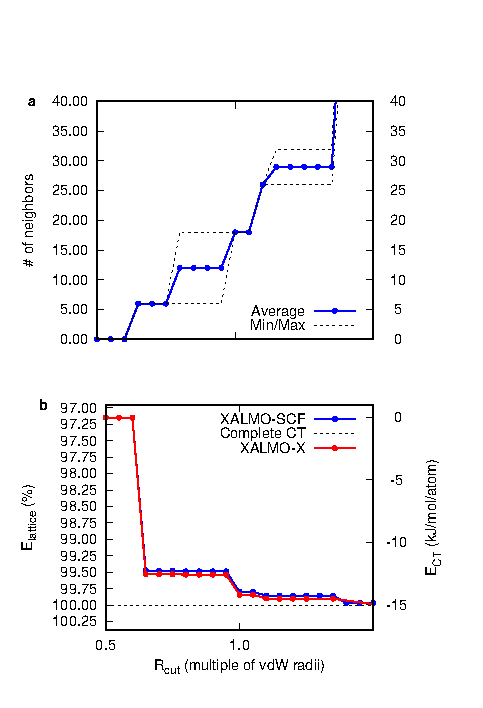
\includegraphics[scale=1]{./plots/LiF_EvR}
\caption{LiF}
\label{lif}
\end{figure}

\begin{figure}
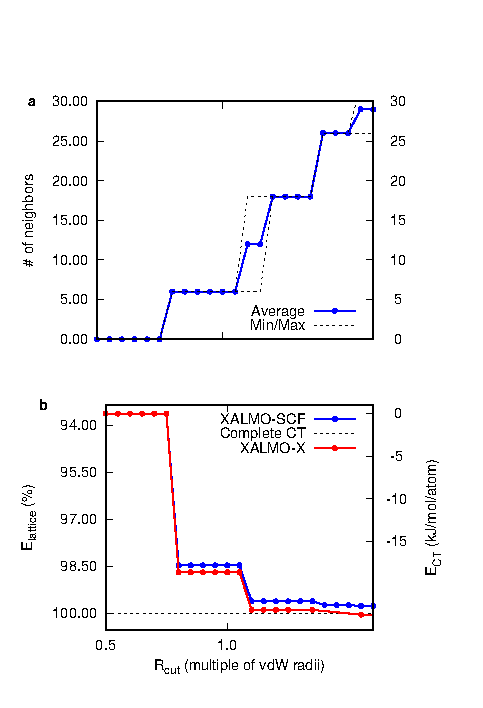
\includegraphics[scale=1]{./plots/LiI_EvR}
\caption{LiI}
\label{lii}
\end{figure}

\begin{figure}
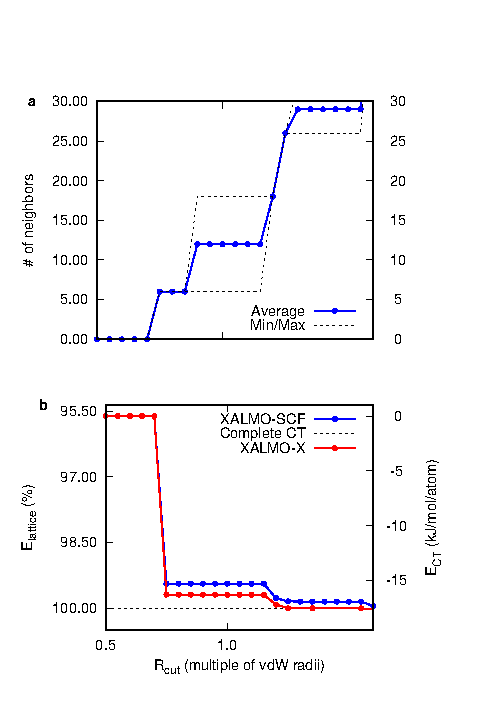
\includegraphics[scale=1]{./plots/NaCl_EvR}
\label{nacl}
\caption{NaCl}
\end{figure}

\begin{figure}
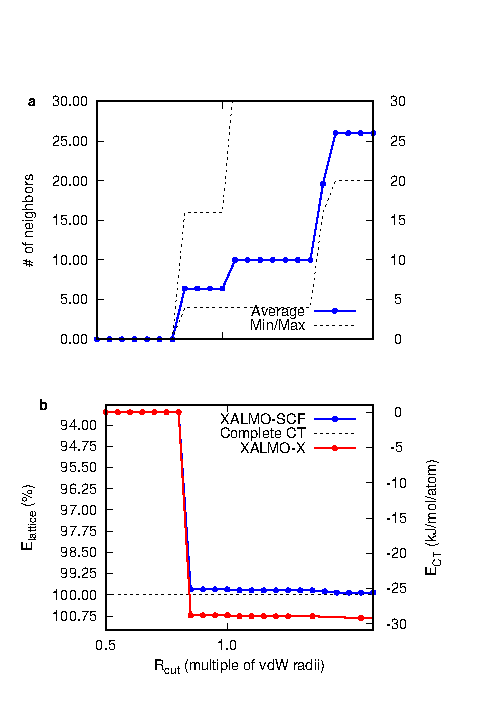
\includegraphics[scale=1]{./plots/RbF_EvR}
\label{rbf}
\caption{RbF}
\end{figure}

\begin{figure}
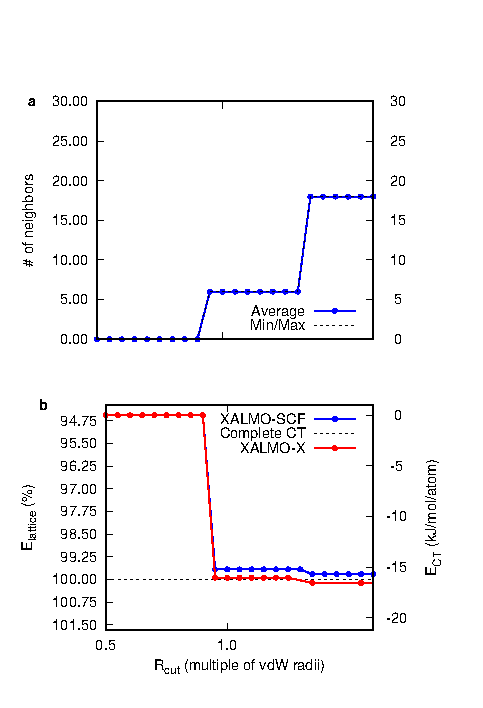
\includegraphics[scale=1]{./plots/RbI_EvR}
\caption{RbI}
\label{rbi}
\end{figure}




\subsection*{ $\text{MgH}_{2}$ }

The binding properties of magnesium hydride have garnered considerable research interest as it is considered one of the most promising materials for cheap hydrogen storage\cite{Hstorage}.  
As such, the charge density inside the crystal's different polytypes has been studied for over four decades\cite{oldmgh2} and some disagreement remains on the degree of ionicity exhbited by the system under its different forms.  
Indeed, nearly all recent results agree that Mg is almost fully ionized to its formal charge +2, yet consensus still has not been reached on the charge density around H in this system\cite{[conflicting DFT/exp sources]}.

We used ALMO DFT to estimate the degree to which the electrons are localized near their resective ions in this crystal and the contribution of CT effects to the cohesive forces keeping the ions bound together.    
The cell parameters for this system were optimized on a lattice of $N = 72$ atoms ($2\times 2\times 3$ unit cells), using a mesh of $2\times 2\times 2\: k$-points, sampled following the Monkhorst-Pack scheme\cite{kpts}.\\ 
Energy calculcations were run on a system of $N = 576$ atoms ($4\times 4\times 6$ unit cells) without using $k$-points.
The cell parameters obtained from the optimization were $a = b = 4.532\angstrom$, $c = 3.007\angstrom$.
The electron density was cutoff at 300 Ry. 
The pseudopotential used to model magnesium's core electronic/nuclear charge only took two core electrons (instead of ten in total) into account to improve convergence.
 
\begin{figure}
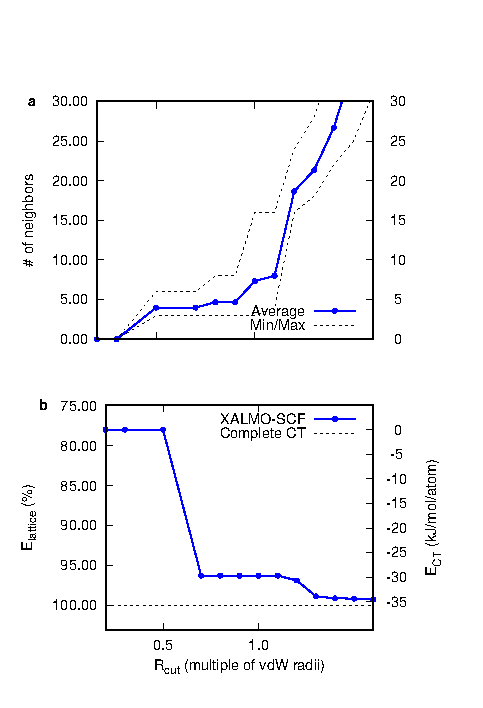
\includegraphics[scale=1]{plots/MgH2_EvR}
\caption{$\text{MgH}_{2}$}
\label{mgh2}
\end{figure}

ALMO-DFT on this system reveals that assuming a completely ionic character for the Mg-H bond yields a surprisingly high 96.40\% of the crystal's overall lattice energy.  
Increasing $R_{cut}$ just enough so that each ion can only interact with its closest neighbours lowers the calculated lattice energy by 29.69 kJ/mol/atom, which accounts for 82.98\% of the system's full CT energy.
As with the alkali halides, we find that CT effects represent a small fraction of the overall binding energy in the solid and only considering nearest neighbour CT effects furthermore recovers the quasi-totality of $E_lattice$ (roughly 99.39\%).
However when considering the fraction of $E_{\text{CT}}$ obtained when only accounting for nearest-neighbour interactions, we
This suggests that the fully relaxed electronic structure of this crystal allows for notable CT between ions and some of their more distant neighbours.
Further evidence of $\text{MgH}_{2}$ strong ionic character is  
%Further doubling the average number of neighbours each ion can interact with only brings us to 85.77\% of $E_{CT,full}$.
%Comparing this to a textbook ionic compound like NaCl, where we found that interaction with first neighbours covered 81.57\% of $E_{CT,full}$ and similarly doubling the number of neighbours gets us to 
%However, increasing the number of neighbours each ion can interact with only marginally lowers the lattice energy. 
This goes to show the degree to which the charge density is localized in this crystal; despite the importance of CT effects between an ion and its immediate neighbours, representing the electronic distribution as completely diffuse only brings marginal improvements to the accuracy of our calculation. 
%This seems to corroborate results like those obtained by Ohba \embh{et al.} using  which estimated the ionic charge on H to be -0.26 at $T = 0\text{K}$ and found the charge density around it to be much more diffuse.
%[IONIC WITH DIFFUSE CHARGE DENSITY NEAR H]


\subsection*{$\text{TiO}_{2}$}


The properties of metal oxides have been the subject of rapidly growing interest, due to the variety of their applications from fields like catalysis to photovoltaic power generation. 
Titanium dioxide is a popular model used to study such compounds due to its experimental convenience (ready supply, high surface quality) and simple structure.
As such, a wide array of \emph{ab-initio} and experimental techniques have been used to study it and all agree on its key characteristics.
$\text{TiO}_{2}$ is characterized as an ionic crystal yet in its most stable forms, rutile and anatase, it has been shown to exhibit strong covalent character\cite{}.
Indeed, the formal on charge on Ti in $\text{TiO}_{2}$ is +4 which, given the high ionization energy of Ti into $\text{Ti}^{4+}$ and the stability of $\text{TiO}_{2}$ in crystalline form, suggests that the ionic model is unsuited for this compound.
Despite, the conduction band being dominated by 
This known Ti-O bond hybridization makes $\text{TiO}_{2}$ an interesting system in which to study CT effects. \\

We ran ALMO-DFT calculations on a lattice of $N = 576$ atoms (same as for magnesium hydride: $4\times 4\times 6$ u.c.), with an electronic density cutoff of 1000 Ry. We only considered rutile stoichiometric $\text{TiO}_{2}$ which is one of its most stable manifestations.\\
The relaxed lattice parameters used for energy calculations were $a = b = 4.715\angstrom$ and $c = 3.034\angstrom$.\\


\begin{figure}
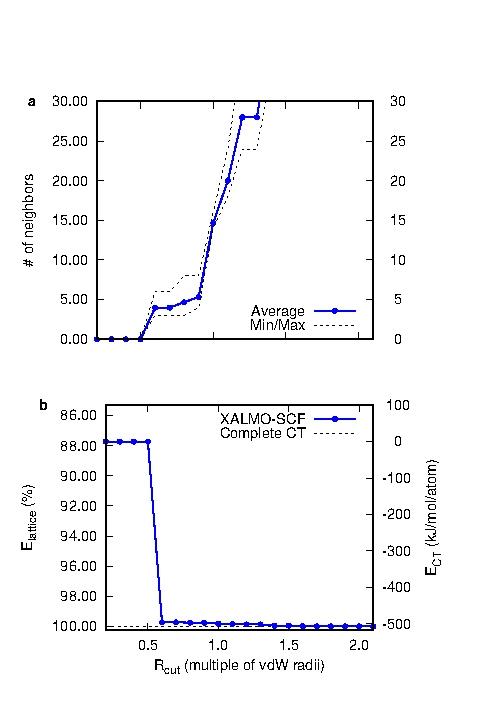
\includegraphics[scale=1]{plots/TiO2_EvR}
\caption{$\text{TiO}_{2}$}
\label{tio2graph}
\end{figure}

Figure \ref{tio2graph} shows us that CT effects account for 57.03\% of the crystal's lattice energy, while only allowing local CT between ions and their immediate neighbours recovers 98.76\%.
%This seems charactersistic of bonds with strong covalent character, which are usually modelled as allowing electrons to move from a fragment to one of its immediate neighbours, but no further.
This is consistent with the intuitve description of a covalent bond as a pair of electrons localized between an atom and its close neighbours. While the quantum mechanical description of a covalent bond is still spatially diffuse, it still predicts that the electrons that compose the bond are extremely likely to remain close to the bound atoms.
Another argument for the covalence of the Ti-O bond in $\text{TiO}_{2}$ is the fact that allowing valence electrons to only move between an ion and its closest neighbours further recover 97.82\% of the CT terms in the overall energy lowering. 
This goes to show that the quasi-totality of the interfragment CT responsible for stabilizing the system is done between neighbouring atoms, similarly to covalently-bonded molecular systems. 
Thus, not only do CT effects play a major role in the electronic structure of this system, but they also mainly take place between immediate neighbours. 
This is compeleltely congruous to the literature's current understanding of this compound's bulk electronic structure.\\

While these results seem qualitatively similar to what was obtained for magnesium hydride, it is worth noting the total (i.e. allowing full delocalization) value of $E_{CT}$ for $\text{TiO}_{2}$ is roughly 500 kJ/mol/atom which is more than ten times what was found for $\text{MgH}_{2}$.
CT also terms represent a much larger proportion of the energy lowering in $\text{TiO}_{2}$ than in $\text{MgH}_{2}$.
Finally, the nature of interfragment seems to be different in both compounds. In $\text{MgH}_{2}$, only ~80\% of CT energy recovered by first-neighbours delocalozation; in TiO2 its ~97\%.

  





[PLOT CONV WRT ITERATIONS]

%However $\text{TiO}_{2}$ also served to study the scalability of our calculation  methods with respect to system size. For such runs, a new algorithm was implemented to invert the overlap matrix which relied on matrix Taylor expansion. Outlined here is a heuristic explanation of the procedure, assuming we are trying to invert the Hermitian matrix $M\in\C^{n\times n} (n\in\N)$.







%First, let $M = A + B$ where $A$ corresponds to $M$'s diagonal elements. Assuming all of $M$'s eigenvalues are nonzero, we can invert $A$ simply by taking the reciprocal of its entries (which all lie along its diagonal): $A^{-1}_{j,j} = (A_{j,j})^{-1}$ (for $1\le j \le n$). We get:

%\begin{align*}
%M = A (\mathbb{I} + A^{-1}B) \implies M^{-1} &= [A (\mathbb{I} + A^{-1}B)]^{-1} \\
%&= (I + A^{-1}B)^{-1} A^{-1}
%\end{align*} 

%The Frobenius norm of matrix $M\in\C^{n\times n}$ is defined as:

%\begin{equation*}
%\norm{M} \vcentcolon=\sqrt{\sum_{i,j}^{n} \mid M_{i,j} \mid ^{2}}
%\end{equation*}

%Assuming that $A^{-1}B$ is diagonalizable and $\mid\lambda_{i}\mid < 1 (1\le i\le n)$ where $\lambda_{i}$ denotes $A^{-1}B$'s $i^{th}$ eigenvalue, we can expand $(\mathbb{I} + A^{-1}B)^{-1}$ the same way one can expand 
%$f(z) = \frac{1}{1+z}$ about $z_{0} = 0$, where $\mid z \mid < 1$\cite{matrixfunc};

%\begin{equation*}
%M^{-1} = \Big(\sum_{k=0}^{\infty} (-1)^k \,(A^{-1}B)^k \Big) A^{-1} = A^{-1} - A^{-1}BA^{-1} + A^{-1}BA^{-1}BA^{-1} - \ldots
%\end{equation*}
 
%In practice the infinite sum is truncated at some $N\in\Ns$, therefore the resulting matrix is usually not the exact inverse $M^{-1}$. It is however possible to get a quantitative measurement of the accuracy this truncated estimate (denoted $M^{-1}_{N}$) by calculating the error $E_{N} = \norm{\mathbb{I} - M^{-1}_{N}\, M}$, where $\norm{\cdot}$ denotes a matrix norm. Assuming all the conditions mentioned above hold, we must have $E_{N}\xrightarrow[N\to\infty] \, 0$. \\



\subsection*{BN}

Boron nitride crystallizes in polymorphs that are structurally similar and isoelectronic to carbon crystalline phases. 
%It also exhibits high chemical and thermal stability thus making applicable in a variety of contexts.
Consequently, cubic BN (c-BN, or borazon[cite og]) resembles diamond in structure and exhibits comparable hardness, but also presents higher thermal and chemical stability, thus revealing its wide potential applicability.
Despite these similarities, bonding in diamond is widely charcterized as purely covalent while BN has been found to display more hybrid ionic-covalent characteristics.
Borazon therefore presents good testing grounds for the ALMO code as, like $\text{MgH}_{2}$ and $\text{TiO}_{2}$, its bonding structure requires a nuanced description.

Implementing ALMO DFT on BN proved to be much less successful than on the previously described systems; table \ref{bngraph} shows that increasing the localization radius of valence electrons, thus allowing the ALMO-obtained charge density to further relax to its natural state, \emph{increases} the energy of the crystal.
This highly unexpected behaviour is due to the lack of convergence of the calculations in this context. 
Figure \ref{convgraph} shows the norm of the energy gradient as CP2K iteratively minimizes the energy (conjugate gradient method with Dai-Yuan conjugator was used in both cases). 
Converging calculations tend to have a monotonically decreasing $\|\nabla E\|$ until it falls below a certain threshold value and ends the minimzation. 
On the other hand, we can see that in the energy minimization of c-BN, $\|\nabla E\|$ fluctuates greatly and does not fall below a certain value.
Close examination of the graph in fact shows that the calculations BN initially converge very fast, before $\|\nabla E\|$ suddenly blows up.
The first part ALMO DFT calculations corresponds to the optimizing the system's electronic structure without allowing interfragment CT, and in doing so, the calculation of the frozen density and polarization energy lowering. 
The second step consists in further relaxing this localized electronic structure by allowing electrons to remain within the region delimited by $R_{cut}$.
It is often this latter part of the computation that fails to converge.
Unconverged calculations usually result in overestimating the final energy (thus \emph{underestimating} the energy \emph{lowering}), as we are evaluating it variationally.


[block diagonal ALMOs converge fast, XALMOs fail (you can notice it on graph)]
[much more densely packed than other crystals we modelled]

\begin{figure}
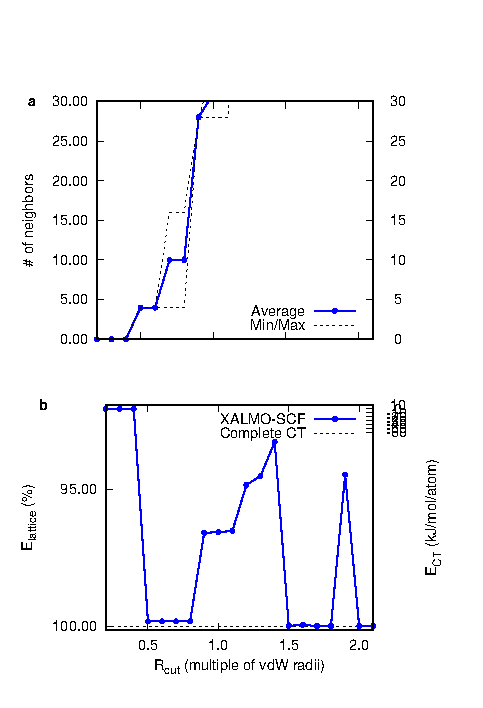
\includegraphics[scale=1]{plots/BN_EvR}
\caption{BN}
\label{bngraph}
\end{figure}





%\begin{figure}[htb]
%\begin{minipage}{0.4\textwidth}
%\begin{tikzpicture}
%  \node (img)  {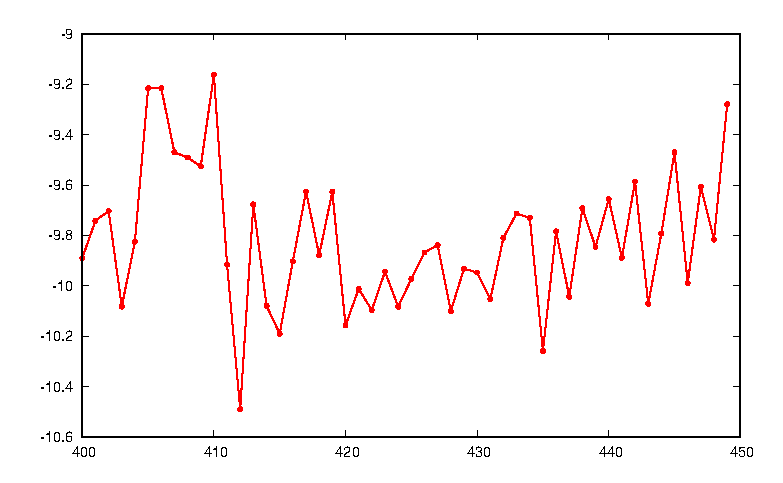
\includegraphics[scale=0.225]{plots/BN_conv_end.eps}};
%  \node[below=of img, node distance=0cm, yshift=1cm,font=\color{red}] {\# iterations};
%  \node[left=of img, node distance=0cm, rotate=90, anchor=center,yshift=-0.7cm,font=\color{red}] {$\|\nabla G\|$};
% \end{tikzpicture}
%\end{minipage}%
%\begin{minipage}{0.4\textwidth}
%\begin{tikzpicture}
%  \node (img)  {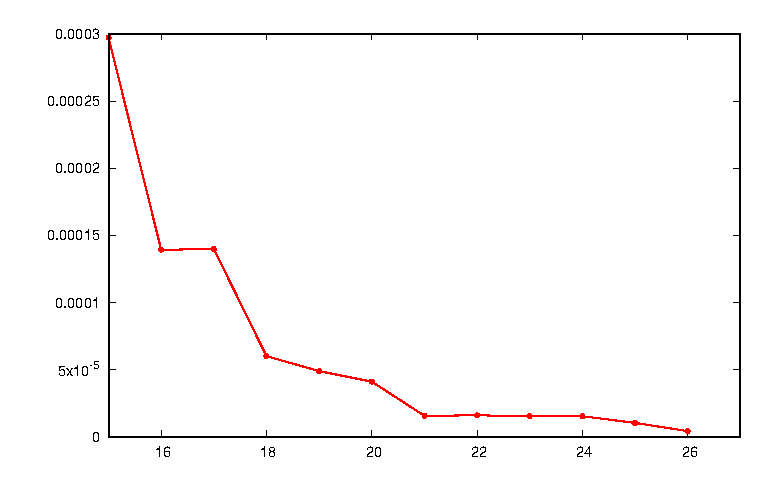
\includegraphics[scale=0.225]{plots/TiO2_conv_end.eps}};
%  \node[below=of img, node distance=0cm, yshift=1cm,font=\color{red}] {\# iterations};
%  \node[left=of img, node distance=0cm, rotate=90, anchor=center,yshift=-0.7cm,font=\color{red}] {$\|\nabla G\|$};
%\end{tikzpicture}
%\end{minipage}%
%\end{figure}

\begin{figure}[htb]
\begin{tikzpicture}
  \node (img1)  {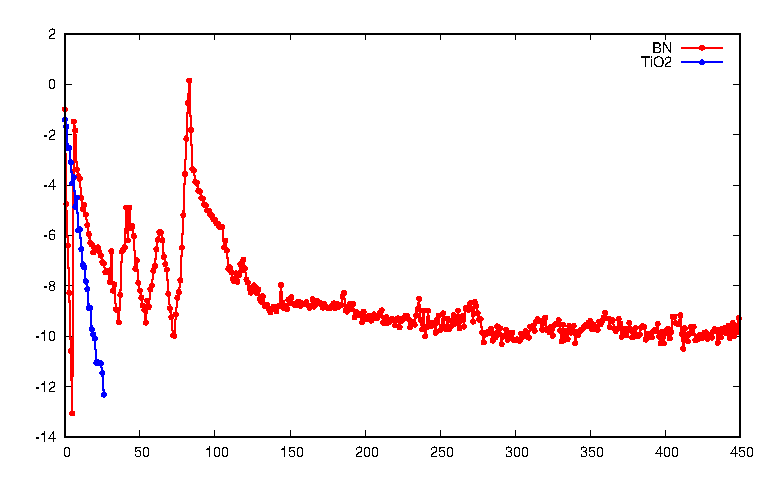
\includegraphics[scale=1.00]{plots/conv_log.eps}};
  \node[below=of img1, node distance=0cm, yshift=1cm] {\# iterations};
  \node[left=of img1, node distance=0cm, rotate=90, anchor=center,yshift=-0.7cm] {ln($\|\nabla E\|$)};
\end{tikzpicture}
\caption{Convergence vs number of iterations for BN and $\text{TiO}_{2}$.}
\label{convgraph}
\end{figure}


\section*{PbSe}
CdSe or other small gap semiconductor   

\section{Conclusions} 

In this paper we aimed to restrain electronic delocalization in our DFT calculations with the following goals:
\begin{enumerate}
\item{Gain further insight on the role of CT effects in different materials}
\item{Implement a linear scaling DFT method on systems where electrons are known to be localized}
\end{enumerate}
The results obatined using the ALMO scheme in our energy calcuations yielded results conistent with the current understanding of bonding in all systems we studied; weakly interacting solids with strong ionic character did not yield high values of $E_{CT}$ and conversely, CT effects played an important for systems known to be more covalent.
However, an important that deserves highlighting is that the ALMO method is best suited for systems like titania; systems exhibiting a notable amount of interfragment CT but a localized electron distribution. 
Indeed, restricting valence electrons to the confines of an ion's immediate neighbourhood yielded very accurate results, and only slightly loosening such constraints gives energies that quasi-identical to those obtained through traditional KS DFT methods. 
Enforcing locality upon the electronic states ensures sparcity of the matrices being manipulated in calculations and dramatically increases the efficiency of such calculations on large systems ($N\geq 1000$ atoms).
Our study of boron nitride revealed 
[Part about BN still being problematic]
[Timing part]
[CT lowering roughly the same for everyone past certain pt?]
[ALMO = promising but doesnt work for certain types of systems; set things up for next paper]



\textbf{Acknowledgments.} The research was funded by the Natural Sciences and Engineering Research Council of Canada through the Discovery Grant. The authors are grateful to Compute Canada and McGill HPC Centre for computer time.

%\textbf{Supporting Information}
%Calculated radial distribution functions of liquid water, comparison of timing benchmarks for the DZVP and TZV2P basis sets, timing benchmarks for systems containing 32,768 water molecules, timing benchmarks for the Kohn-Sham matrix build. This material is available free of charge via the Internet at http://pubs.acs.org.

\bibliography{almo-expand}
%\bibliography{methods}

\end{document}
